\documentclass[12pt]{article}

\usepackage{amsmath}
\usepackage[dvips]{graphicx}
\usepackage{natbib}
\usepackage{url}

\renewcommand{\contentsname}{CONTENTS}
\renewcommand{\refname}{BIBLIOGRAPHY}

\bibliographystyle{apa}

\begin{document}

\title{
\includegraphics[width=0.2\textwidth]{agflogo} User Guide}
\author{Peter Mills\\\textit{peteymills@hotmail.com}}

\maketitle

\begin{center}
	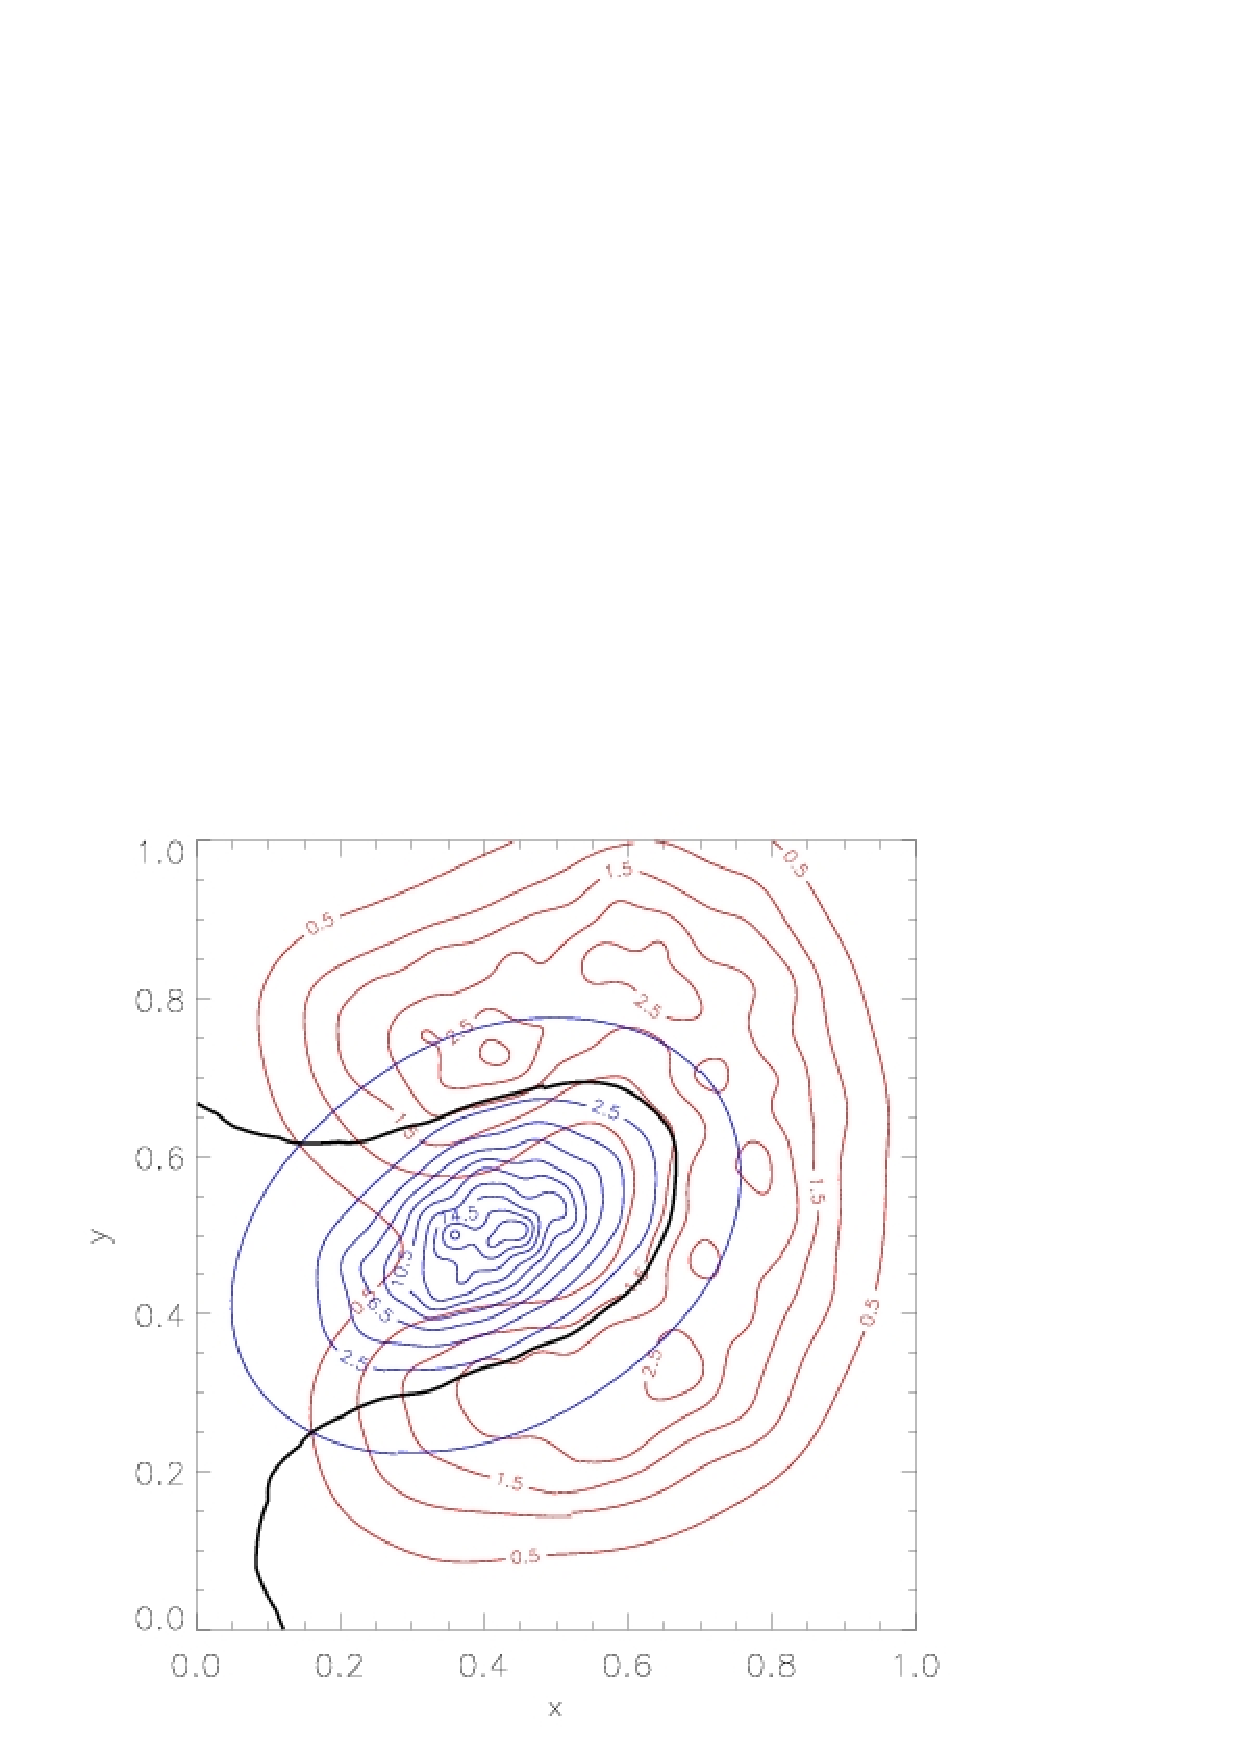
\includegraphics[width=0.65\textwidth]{sc}
\end{center}

\newpage

\tableofcontents

\newpage

\section{INSTALLATION}

  First, make sure you have the required dependencies.  You will need the {\it GNU Scientific Library (GSL)}.  If it is not already installed on your system, download and install it.  Take note of the location of the compiled libraries and include files.  You will also need to install {\it libpetey}, another, much smaller numerical library--this now comes bundled with libAGF.

  Download the source from Github (\url{https://github/peteysoft/libmsci}) or your favourite mirror.  Unzip and unpack the tarball to the desired directory.  Modify the makefile with the appropriate directories, compiler names and compiler flags.  Type \verb"make" from inside the libagf directory to perform the build and \verb"make install" to copy the executables, libraries and include files to the appropriate directories.

  A configure script is not supplied: please refer to the Peteysoft coding standards \verb\coding_standards.txt\ in the base of the installation directory (\url{https://github.com/peteysoft/libmsci/blob/master/doc/coding_standards.txt}).

  Make sure the following macros have been set properly in the make file:

\begin{tabular}{ll}
	\verb/LIB_PATH/ = & location of your compiled libraries\\
	\verb/BIN_PATH/ = & location of binary executables\\
	\verb/INCLUDE_PATH/ = & location of your include files\\
	& \\
\verb/GSL_LIB/ = & location of the GSL libraries (if different from above)\\
\verb/GSL_INCLUDE/ = & location of the GSL include files (if different from above)\\
		     & \\
	\verb/CC/ = & name of your C++ compiler
\end{tabular}

  There are two ways to change the optimisation of the binaries.  If you would like multiple versions with different levels of optimisation, be sure to change the OPT\_VER macro.  This will append the optimisation flag to all the object files, libraries and executables.  If you only want one version, then modify the CFLAGS macro in the usual manner.

  To test the resulting executables, type, \verb"make test".  To see the resulting comparison summary, it may be necessary to type it twice.  Overall accuracies of all the classification algorithms should be around 90 \% and the uncertainty coefficients should be over 0.5, while the confidence ratings should roughly match the accuracies.  When comparing one algorithm to another, accuracies should be around 99\% and uncertainty coefficients around 0.92, while the confidence ratings should be 1. or close to it, regardless of accuracy.  Probability density comparisons should be around $r=\lbrace 0.98, 0.99, 0.97, 0.99 \rbrace$ for KNN and AGF for the first class and KNN and AGF for the second class, respectively.

\section{FILE FORMATS}

  The programs accept three types of files with very simple, binary formats.  Although portability is sometimes an issue, the binary formats are easy to generate and allow for rapid access and compact storage.  For vector data, use the extension, \verb".vec".  Vector files have a four byte header (by default, see next paragraph) that indicates the dimensionality of the data.  After that, each vector is stored one after the other as arrays of four byte floats.  To write such a file in C++, you can use the following commands:

\begin{verbatim}
#include <stdio.h>
#include <stdint.h>

int main() {

  FILE *fs;

  float ** data;	//array of vectors
  int32_t n;		//number of vectors
  int32_t D;		//number of dimensions

  n=100;	//(e.g.)
  D=2;

  data=new float * [n];
  for (int32_t i=0; i<n; i++) data[i]=new float[D];

  //... commands to fill the matrix ...

  fs=fopen("data.vec", "w");
  fwrite(&D, sizeof(D), 1, fs);
  for (int32_t i=0; i<n; i++) fwrite(data[i], sizeof(float), D, fs);
  fclose(fs);
  
  for (int32_t i=0; i<n; i++) delete [] data[i];
  delete [] data;

}
\end{verbatim}

In IDL (Interactive Data Language):

\begin{verbatim}
  n=100		;(e.g.)
  d=2		;(e.g.)
  data=fltarr(d, n)
  ;... commands to fill the matrix ...
  openw, 1, "data.vec"
  writeu, 1, d, data
  close, 1
\end{verbatim}

In Fortran:

\begin{verbatim}
  parameter(n=100)
  parameter(d=2)
  real data(d, n)

  ...

  open(10, file="data.vec", form="binary")
 
  write(10) d
  do j=0, n
    write(10) (data(i, j), i=1,d)
  enddo

  close(10)
\end{verbatim}

For scalar data, the programs use a straight binary dump of the data.  By default, four byte (32 bit) integers are used for class data and four byte (32 bit) floating point variables are used for continuous data. (To change the types used by the command-line programs, edit the header \verb/agf_defs.h/.) For class data, use the extension \verb".cls" and for floating point data, use the extension, \verb".dat".  Scalar data always corresponds to vector data and is ordered accordingly.


To write such data in C++, you can use the following commands:

\begin{verbatim}
#include <stdio.h>
#include <stdint.h>

int main() {
  FILE *fs;
  int32_t *data;
  int32_t n;

  n=100;	//(e.g)
  data=new long[n];
  //... commands to fill array  ...
  fs=fopen("data.cls", "w");
  fwrite(data, sizeof(int32_t), n, fs);
  fclose(fs);
  delete [] data;
}
\end{verbatim}

In IDL:

\begin{verbatim}
  data=lonarr(100)
  ;...
  openw, 1, "data.cls"
  writue, 1, data
  close, 1
\end{verbatim}

In Fortran:

\begin{verbatim}
  parameter(n=100)
  integer data(n)

  ...

  open(10, file="data.cls", form="binary")
 
  write(10) (data(i), i=1,n)

  close(10)
\end{verbatim}

Note that the class indices must go from 0 to $N_c-1$, where $N_c$ is the number of classes.  The classification routines will output two binary files containing scalar data:  one with the extension, \verb".cls" containing class estimates, and one with the extension \verb".con" containing ``confidence ratings'' which are simply conditional probabilities re-scaled in the following manner:
\begin{equation}
c = \frac{N_c P(c | \vec x) - 1}{Nc - 1}
\end{equation}

where $P(c | \vec x)$ is the conditional probability of the ``winning'' class.  A confidence rating of one indicates theoretically perfect knowledge of the true class, while a value of zero indicates that the result is little better than chance.  If conditional or joint probabilities are needed for all the classes, they are written to standard out.

To read the output files, examine the routines \verb"read_clsfile" for reading class data, \verb"read_vecfile" for reading vector data and \verb"read_datfile" for reading scalar floating point data, contained in the source file, \verb"agf_util.cc", or you can use them directly.  Note that vector data is allocated in one contiguous block, meaning that it can also be read and written in one contiguous block.  It can also be deleted very simply using two commands:

\begin{verbatim}
  float ** data;
  nel_ta n;
  dim_ta D;

  data=read_vecfile(data, n, D);

  delete [] data[0];
  delete [] data;
\end{verbatim}

In addition, the {\it sparse} satellite library contains a utility called \verb/sparse_calc/ that can operate on both types of binary files containing floating point data (but not class data).  To read in and print a file of vector data called, \verb"foo.vec" type the following commands:

\begin{verbatim}
$>sparse_calc
%s%c>print full(foo.vec)
\end{verbatim}

To read in and print a file of scalar data called, \verb"bar.dat", type the following:

\begin{verbatim}
%s%c>print vector(bar.dat)
\end{verbatim}

Some users may prefer to use ASCII file formats to store their data.  If this is the case, there are a number of file conversion utilities included for comparison with other algorithms.  See Section \ref{COMMAND_LINE_EXECUTABLES}, COMMAND LINE EXECUTABLES.

Sometimes it's desireable to normalize the data before performing classifications.  Normalization in libagf has now been generalized to linear transformation and includes singular value decomposition as well as feature selection.  The command, \verb"agf_precondition", is used to perform linear transformations on test and training (features) data and store the resulting transformation matrix in the same binary format for vector data as described above.  The default name is the same as before with the extension \verb".std" appended to the output base file name.  Features data can still be transformed directly within the machine learning routines using the command options \verb"-n", \verb"-S" and \verb"-a": see Section \ref{COMMAND_PARAMETERS}, COMMAND PARAMETERS.  By default, pre-trained model data is stored in the normalized coordinates; to store it in the non-normalized coordinates, use the command switch, \verb"-u".

\section{COMMAND PARAMETERS}

\label{COMMAND_PARAMETERS}

Most of the commands have the following syntax:

\begin{verbatim}
command [options] model [test_data] output
\end{verbatim}

where \verb\model\ is the base name of the files containing either a set of training data or a pre-trained model, \verb/test_data/ is the file containing test data and output is the base name of the files in which to store the final estimates.

To get a summary of the syntax and parameters, simply type the command name with no arguments, e.g.:

\begin{verbatim}
> classify_b
Syntax:   classify_b [-n] [-u] [-a normfile] border test output

where:
  border      files containing class borders:
                .brd for vectors
                .bgd for gradients
                .std for variable normalisations (unless -a specified)
  test        file containing vector data to be classified
  output      files containing the results of the classification:
                .cls for classes, .con for confidence ratings

options:
  -n          option to normalise the data
  -u          normalize borders data (stored in un-normalized coords)
  -a normfile file containing normalization data
\end{verbatim}

Here is a list of all the options, although not all commands support all options:

\begin{tabular}{ll}
Option & Function \\
\hline
-- & External command to train a binary classifier.\\
-+ & Extra options to pass to binary training command.\\
-\^ & External command to convert data formats for above.\\
-0 & Read from stdin.\\
-1 & Write to stdout.\\
-a & Name of file containing normalization data.\\
-A & Use ASCII files instead of binary.\\
-b & Short output (\verb/cls_comp_stats/)\\
-B & Sort by class/ordinate.\\
-c & Algorithm selection:\\
& nfold cross-validation:\\
& \verb/  /0=AGF borders (default) classification\\
& \verb/    /1=AGF classification\\
& \verb/    /2=KNN classification\\
& \verb/    /3=AGF interpolation\\
& \verb/    /4=KNN interpolation\\
& \verb/    /5=AGF borders multi-class\\
& \verb/  /PDF validation:\\
& \verb/    /6=AGF PDF estimation\\
& \verb/    /7=KNN PDF estimation\\
-C & No class data.\\
-d & Number of divisions in cross-validation scheme.\\
-D & Generate ROC curve by varying the discrimination border.\\
-e & Return error estimates.\\
-E & Value for missing data.\\
-f & For validation schemes:  fraction of training data to use for \\
   & testing.\\
-F & Select features.\\
-g & Use lograthmic progression. \\
-h & Relative difference for calculating numerical derivatives.
\end{tabular}

\begin{tabular}{ll}
-H & Omit header data.\\
-i & Class borders: maximum number of iterations in supernewton.\\
-I & Weights calculation: maximum number of iterations in supernewton.\\
-j & Print joint instead of conditional probabilities to stdout.\\
-k & Number of k-nearest-neighbours to use in the estimate\\
-K & Keep temporary files (do not delete on exit).\\
-l & Tolerance of W.\\
-L & Floating point ordinates.\\
-m & Type of metric to use.  Only works for knn classification.\\
-M & Get min. and max./LIBSVM format.\\
-n & Takes averages and standard deviations of the training data and \\
 & normalizes both the training and test data.\\
-N & Maximum number of iterations in supernewton.\\
-o & Name of log file.\\
-O & External command for binary classification prediction.\\
-p & Threshold density in clustering algorithm.\\
-P & Calculate correlation/covariance matrix.\\
-q & Number of trials/divisions.\\
-Q & Algorithm selection:\\
  & \verb/  /optimal AGF: how to calculate the filter variances\\
  & \verb/    /0=halving max filter variance (default);\\
  & \verb/    /1=filter variance min and max;\\
  & \verb/    /2=total weight min and max\\
  & \verb/  /non-hierarchical multi-class classification:\\
  & \verb/    /0=constrained inverse (not always optimal)\\
  & \verb/    /1=linear least squares, no constraints or re-normalization\\
  & \verb/    /2=voting from pdf, no re-normalization\\
  & \verb/    /3=voting from class label, no re-normalization\\
  & \verb/    /4=voting from pdf overrides least squares, conditional\\
  & \verb/      /probabilities are adjusted and re-normalized\\
  & \verb/    /5=voting from class overrides least squares, conditional\\
  & \verb/      /probabilities are adjusted and re-normalized\\
  & \verb/    /6=experimental\\
  & \verb/    /7=constrained inverse (may be extremely inefficient)
\end{tabular}

\begin{tabular}{ll}
-r & Class borders: value of conditional prob. at discrimination border.\\
-R & For random sampling.\\
-s & Number of times to sample the class border.\\
-S & Singular value decomposition: number of singular values to keep.\\
-t & Desired tolerance when searching for class borders.\\
-T & Class threshold for class-borders calculation.\\
-u & Store borders data in non-normalized coordinates.\\
-U & Re-label classes to go from $[0, nc)$.\\
-v & First filter variance bracket.\\
-V & Second filter variance bracket/initial filter variance.\\
-w & Lower bound for W in AGF optimal/constraint weight\\
-W & Parameter Wc--equivalent to k in a k-nearest-neighbours scheme.\\
  & See paper describing the theory.\\
-x & Run in background.\\
-X & Ratio between sizes of sample classes ($P(2)/P(1)$).\\
-z & Randomize data.\\
-Z & In-house LIBSVM codes.
\end{tabular}

\section{COMMAND LINE EXECUTABLES}

\label{COMMAND_LINE_EXECUTABLES}

This is a list of commands and their function:

\subsection{Direct routines}

Direct, non-parametric classification, interpolation/regression, pdf estimation using variable-bandwidth kernel estimation:

\begin{tabular}{ll}
\verb/agf/ & Uses adaptive Gaussian filtering\\
\verb/knn/ & Uses k-nearest neighbours
\end{tabular}

  All the direct kernel estimation operations have been collected into two executables: one for AGF called, \verb"agf", and one for k-nearest-neighbours called, \verb"knn".  Both of them take an extra argument which specifies which operation to perform: \verb"classify", \verb"interpol" or \verb"pdf".

\subsection{Binary classification}

Two-class classification by training a model:

\begin{tabular}{ll}
\verb/class_borders/ & Searches for the class borders using AGF.\\
\verb/classify_b/ & Performs classifications using a set of border samples.
\end{tabular}

\subsection{Multi-class classification}

Multi-class classification using a series of class-borders:

\begin{tabular}{ll}
\verb/multi_borders/ & 	Trains a multi-class model based on a control file.\\
\verb/classify_m/: & Performs classifications using model output from \verb/multi_borders/.\\
\verb/svm_accelerate/: & Trains a multi-borders model from a native LIBSVM model.
\end{tabular}

  Multi-borders classification represents a significant step forward with this library.  The operation of these programs, called from the command line using \verb/multi_borders/ and \verb/classify_m/ is quite involved and is described in detail in Section, \ref{MULTI_BORDERS_CLASSIFICATION}, MULTI-BORDERS CLASSIFICATION.

\subsection{Testing/validation}

\begin{tabular}{ll}
\verb/cls_comp_stats/ &	Calculates the accuracy of classification results.\\
\verb/nfold/ &	Performs n-fold cross-validation for the three different \\
		    & classification algorithms or for the interpolation routines.\\
\verb/agf_preprocess/: & Splits a dataset for validation schemes.\\
\verb/pdf_sim/ & Generates a synthetic dataset with the same approximate \\
		      & PDF as the training data.\\
\verb/validate_pdf.sh/ & Validates probability density function (PDF) estimates.\\
\verb/agf_correlate/ & Correlates two binary files containing scalar \\
			    & floating point data.\\
\verb/roc_curve/ & Computes the receiver operatoring characteristic \\
		& (ROC) using three different methods.
\end{tabular}

\subsection{Clustering}

\begin{tabular}{ll}
  \verb/cluster_knn/ & Uses k-nearest neighbours and a threshold density\\
		     & to perform a clustering analysis.  See description, \\
	      & below.\\
  \verb/browse_cluster_tree/ &Create a dendrogram and manually browse through\\
		    & it and assign classes.
\end{tabular}

  The first clustering algorithm works by calculating the density of each training samples.  If the density is larger than a certain threshold, a class number is assigned and the program recursively calculates the densities of all the samples in the vicinity, based on its k neighbours, and assigns the same class number to each if they also exceed the threshold.  Samples lower than the threshold are assigned the class label of 0, while clusters are assigned consecutive values starting at 1.  This is far simpler than a dendrogram, but somewhat less general although the final result should be similar.  But, we've added a dendrogram anyway.

\subsection{Experimental}

\paragraph{Continuum extension}:
Programs that extend the classification algorithms to work with continuous data:

\begin{tabular}{ll}
  \verb/c_borders.sh/ & Trains a continuum classification model.\\
  \verb/classify_c/ & Returns coninuum extension estimates.\\
\end{tabular}

\paragraph{Discrete Bayesian modelling}: programs that model the probability distributions through binning.

\begin{tabular}{ll}
  \verb/sort_discrete_vectors/ & Sorts a set of discrete vectors.\\
  \verb/search_discrete_vectors/ & Searches within a set of discrete vectors and\\
		& estimates the probability density.
\end{tabular}

\subsection{Pre-/post-processing}

\begin{tabular}{ll}
\verb/agf_procondition/ & Performs linear transformations on coordinate (feature)\\
 & data and outputs the transformation matrix.  Normalization, \\
 & singular-value-decomposition (SVD) and feature selection \\
 & are supported.\\
\verb/agf_preprocess/ & Processes both coordinate data and class data.  \\
 & Supports class selection, re-labelling and partitioning, \\
 & file splitting for validation and cross-correlation calculation.
\end{tabular}

\subsection{File conversion}

\begin{tabular}{ll}
\verb/lvq2agf/ & Converts the LVQPAK (ASCII) file format to the binary format \\
 & accepted by libagf.  Many users may find these ASCII formats \\
 & easier to work with.\\
\verb/svm2agf/ & LIBSVM format to libAGF.\\
\verb/svmout2agf/ & Converts (ASCII) output from LIBSVM to binary libAGF format.\\
\verb/agf2ascii/ & Converts binary libAGF format to ASCII (LVQPAK or LIBSVM) \\
			& format.\\
\verb/C2R/ & Converts a two-class classification to a difference in conditional\\
		  & probabilites. The equation is:\\
	& \verb\  \$R = (2 c - 1) C$\\
& where c is the class and C is the confidence rating.\\
\verb/mbh2mbm/: & Collates a multi-file multi-borders model into a single \\
	 	& ASCII file.\\
\verb/float_to_class/: & Converts floating point data into class data by\\
	 	& binning it into discrete ranges.\\ 
\verb/class_to_float/: & Converts class data into floating point. \\
\end{tabular}

The LVQPAK file format is probably the easiest to work with.  There is one header with the number of dimensions, followed by a listing of the vectors, one vector per line, each column is a dimension except for the last one which is the class.  The \verb/sample_class/ program prints its results to standard out in an LVQPAK-compatible format--see Section \ref{EXAMPLES}, EXAMPLES.

\subsection{Commands used by other commands}

  Note that some commands call other commands, therefore these latter commands must be in your path.

\begin{tabular}{ll}
  \verb/agf_precondition/ & Called by all the machine learning programs if one or\\
			  & more of the \verb"-a", \verb"-n" or \verb"-S" switches are used\\
  \verb/pdf_agf/, \verb/pdf_knn/ & still used by \verb/validate_pdf.sh/
\end{tabular}

\subsection{Deprecated}

  \verb/classify_a/, \verb/classify_knn/, \verb/int_agf/, \verb/int_knn/, \verb/test_classify/, \verb/test_classify_b/, \verb/test_classify_knn/

To compile and install older routines, type, \verb"make old".


\section{ERROR CODES AND DIAGNOSTICS}

  All commands will return ``0'' upon successful completion or one of the following error codes:

\begin{tabular}{ll}
Code & Meaning\\
\hline
  1	&	Wrong or unsufficient number of arguments.\\
101	&	Unable to open file for reading.\\
111	&	File read error.\\
256	&	File read warning.\\
303	&	Allocation failure.\\
201	&	Unable to open file for writing.\\
211	&	File write error.\\
512	&	File write warning.\\
401	&	Dimension mismatch.\\
411	&	Sample count mismatch.\\
501	&	Numerical error.\\
511	&	Syntax error.\\
503	&	Maximum number of iterations exceeded.\\
768	&	Parameter out of range.\\
1024	&	Command option parse error.\\
 21	&	Fatal command option parse error.\\
901	&	Internal error.\\
911	&	Other error.\\
1280	&	Other warning.
\end{tabular}

Note that warnings are always divisible by 256 so that when passed back to the command line return a 0 exit status so as not to interupt running scripts.  Error codes are also listed in the include file, \verb"error_codes.h" in the libpetey distribution.  Note that non-fatal errors reduce to '0' if passed to the command line.

  AGF routines also return a set of diagnostics, for example:

\begin{verbatim}
diagnostic parameter               min        max    average

iterations in supernewton:**          4         52       11.8
tolerance of samples:                   0   3.53e-05   2.59e-06

** total number of iterations:     1178
   number of bisection steps:      276
   number of convergence failures: 0


diagnostic parameter               min        max    average

iterations in agf_calc_w:             2          6       3.73
value of f:                       2.6e-13      0.284    0.00146
value of W:                         20.00      20.00      20.00

total number of calls: 1430

\end{verbatim}

  The first parameter indicates the number of iterations required to reach the correct value for the total of the weights, $W$.  For efficiency reasons, this should be as small as possible, however the super-linear convergence of the root-finding algorithm (``supernewton'') means that the brackets can be quite far away without much effect on efficiency.  To change the values of the filter variance used to bracket the root, use \verb/-v/ for the lower bracket and -V for the upper bracket.  Normally the defaults should work just fine but to decrease the number of iterations, they should be narrowed.  If they fail to bracket the root, the offending bracket is pushed outward.  These changes are ``sticky'', so the brackets can, in fact, be set arbritrarily narrow and even quite far from the root.

  To change the tolerance of $W$, use the \verb/-l/ switch.  To change the maximum number of iterations, use the \verb/-i/ or \verb/-I/ switch.

  The second parameter is the number of iterations required to converge to the class border, excluding convergence failures.  This is only applicable when searching for the class borders.  To change the maximum number of iterations (default is 100) in the root-finding algorithm, use the \verb/-i/ or \verb/-N/ parameter.

  The third parameter is the value of the minimum filter weight divided by the maximum and is only applicable when the \verb/-k/ option (selecting a number of nearest neighbours) has been set.  Ideally, it should be as small as possible, although values as large as 0.2 often produce reasonable results.  Be sure to experiment with your own particular problem.  To decrease it, increase the number of nearest neighbours used in the calculations which has the undesirable side effect of increasing computation time.  In general, $k$ should be a fair bit larger than $W$.

  The tolerance of the samples only applies when searching for class borders.  It shows how close the value of $R=P(2|\vec x)-P(1|\vec x)$ (difference in conditional probabilities) is to zero at each border sample.  This is set using the -t option and the diagnostic should be close to the set value.  It is sometimes larger because the convergence test of the root-finding routine looks at tolerance along the independent variable as well as the dependent variable--whichever is better.

  To best understand how to interpret the diagnostics and use these to set the operational parameters, be sure to read the paper entitled, ``Adaptive Guassian Filters: a powerful new method for supervised learning'', in the \verb|doc/| sub-directory of this installation or \citet{Mills2011} which is a more fleshed-out version of it.


\section{MULTI-BORDERS CLASSIFICATION}

\label{MULTI_BORDERS_CLASSIFICATION}

  Multi-borders is an algorithm that generalizes the AGF-borders binary classification algorithm to multiple classes.  It is a means of specifying the configuration of the class borders using a recursive control language.  The \verb/multi_borders/ command is used for training a multi-borders model and has the following syntax:
\begin{verbatim}
    multi_borders [options] control-in train model control-out
\end{verbatim}
where:
\begin{itemize}
\item \verb$control-in$ is the input or training control file; 
\item \verb$train$ is the base-name of the binary files containing the training data
\item \verb$model$ is the base-name for the files that will contain each of the binary classification models and 
\item \verb$control-out$ is the output or classification control file which is passed to the classification program, \verb/classify_m/.
\end{itemize}

\subsection{Multi-borders classification the easy way}

To train a four-class one-versus-one multi-class class borders classification model,
use the \verb/print_control/ command to generate one of several
standard multi-class models and pass it directly to the \verb/multi_borders/
command:

\begin{verbatim}
$>print_control -Q 6 4 | multi_borders foo bar foobar.txt
\end{verbatim}

The training data is contained in \verb/foo/;
the trained binary classification models are output in a series of files (six in this case)
starting with \verb/bar/. The output control file, \verb/foobar.txt/, tells the prediction program,
\verb/classify_m/ how the binary classifiers are configured:
\begin{verbatim}
$>classify_m foobar.txt test.vec results
\end{verbatim}
Where \verb\test.vec\ contains the test points
while the results are stored in \verb"result.cls" and \verb"result.con".
The \verb/-Q/ options determines the multi-class model used:
type \verb/print_control/ with no arguments to get a list of supported models.

\subsection{Multi-borders classification the hard way}

Consider the following control file (\verb/test_multi5.txt/):
\begin{verbatim}
"-s 100" {
  "."      {0 1}
  ""       0 1 / 2;
  "-s 75"  0 / 1 2;
  {
    "-s 50" {2 3}
    4 5
  } 
}
\end{verbatim}
When passed to \verb/multi_borders/ as follows:
\begin{verbatim}
$>multi_borders -n -s 125 test_multi5.txt foo bar foobar.txt
\end{verbatim}
runs the following set of statements:
\begin{verbatim}
agf_precondition -a bar.std -n foo.vec bar.139397543805655.vec
cp foo.cls bar.139397543805655.cls
class_borders -s 100 bar.139397543805655 bar.00 0 / 1
class_borders -s 50 bar.139397543805655 bar.01.00 2 / 3
class_borders -s 125  bar.139397543805655 bar.01-00 2 3 4 / 5
class_borders -s 75 bar.139397543805655 bar.01-01 2 3 / 4 5
class_borders -s 100 bar.139397543805655 bar 0 1 / 2 3 4 5
rm bar.139397543805655.vec
rm bar.139397543805655.cls
\end{verbatim}

Initial versions printed these commands to standard out with running them the
job of the user. Now they are executed directly with the option of 
running them in the background using the \verb"-x" switch.
It is still possible to print out the commands only using the \verb"-0"
or \verb"-K" switch.

The contents of \verb"foobar.txt" are as follows:
\begin{verbatim}
bar {
  bar.00 {
    0
    1 
  }
  bar.01-00 0 1 / 2;
  bar.01-01 0 / 1 2;
  {
    bar.01.00 {
      2
      3
    }
    4
    5
  }
}
\end{verbatim}

Note that each of the names in this file correspond to pairs of files generated by the commands in the previous script. To classify the data in a file named \verb"test.vec" use the following command:

\begin{verbatim}
$>classify_m -n foobar.txt test.vec result
\end{verbatim}

There are two types of multi-borders classification: {\it hierarchical} and {\it non-hierarchical}.  In non-hieararchical multi-borders classification, all the classes are partitioned in multiple ways using a binary classifier and the equations relating the conditional probabilities of each class to those of the binary classifiers are solved returning all of the conditional probabilities.  In the hierarchical method (also called a {\it decision tree}), the classes are partitioned using either a binary classifier or a non-hierarchical multi-classifier, then each of those partions are partitioned again and so on until there is only one class left in each of the partions.  Hierarchical classification returns only the conditional probability of the winning class.  The \verb/classify_m/ method automatical detects whether a control file uses the hierarchical method or only the non-hierarchical method(that is it has only one level) and prints out conditional probabilities as appropriate.  

  The parameters for training each binary classifier are contained in double quotes in the training control file.  To take parameters from the command line, use the null string (\verb/""/) while a period (\verb/"."/) tells the program to use the last set of parameters at the same level or below.  A series of statements for training each of the binary classifiers are generated and executed using the ``system'' command.  Once the commands are run, these binary classifiers will be stored in a pair of uniquely named files, the base-names of which replace, in the final control file, the quoted parameter lists from the training control file.

  In the control language, going up a level in the hierarchical scheme is denoted by a left curly brace (\verb'{') while going down is denoted by a right curly brace (\verb$}$).  In a non-hierarchical model, we specify the parameters (file name) of each of the binary partitions followed by the partitions themselves: two lists of classes separated by a forward slash (\verb'/').  Class labels for non-hierarchical partitions are relative, that is they go from 0 to the number of classes in the non-hierarchical model less one.  Class labels in the top level partitions are absolute, therefore must be unique.  These should also go from 0 to one less than the total number of classes in the over-all model, but need not.

  In this example, there are six classes.  They are first partioned into a group of two and a group of four.  The group of four is partitioned into three parts, the first of which is partitioned into two classes and the second and third of which are single classes. The \verb/print_control/ command can be used to generate common control files.

A good way to understand the ``multi-borders'' paradigm is to look at the example cases in the \verb"examples/humidity" data directory.  There is also a draft paper contained in the \verb"docs/" sub-directory.


%\section{USING MULTI-BORDERS WITH EXTERNAL BINARY CLASSIFIERS}
\subsection{Multi-borders with external binary classifiers}

The multi-borders routines can now interface with external binary classification software, specifically, either LIBSVM, or a pair of programs that have the same calling conventions.  For training, use the \verb"--" switch to pass the command name to \verb/multi_borders/.  Consider the above control file as an example, but without any of the control switches:

\begin{verbatim}
"" {
  ""  {0 1}
  ""  0 1 / 2;
  ""  0 / 1 2;
  {
    "" {2 3}
    4 5
  } 
} 
\end{verbatim}

We pass the LIBSVM command, \verb"svm-train", to \verb"multi_borders", as follows:
\begin{verbatim}
$>multi_borders -M -- "svm-train -b 1" -+ "-h 0 -c 25" \
		test_multi.txt foo.svm bar foobar.txt
\end{verbatim}
which will execute the following statements:
\begin{verbatim}
agf_preprocess -A -M foo.svm bar.00.2367545368.tmp 0 / 1
svm-train -b 1 -h 0 -c 25  bar.00.2367545368.tmp bar.00
rm -f bar.00.2367545368.tmp
agf_preprocess -A -M foo.svm bar.01.00.2367545368.tmp 2 / 3
svm-train -b 1 -h 0 -c 25  bar.01.00.2367545368.tmp bar.01.00
rm -f bar.01.00.2367545368.tmp
agf_preprocess -A -M foo.svm bar.01-00.2367545368.tmp 2 3 4 / 5
svm-train -b 1 -h 0 -c 25  bar.01-00.2367545368.tmp bar.01-00
rm -f bar.01-00.2367545368.tmp
agf_preprocess -A -M foo.svm bar.01-01.2367545368.tmp 2 3 / 4 5
svm-train -b 1 -h 0 -c 25  bar.01-01.2367545368.tmp bar.01-01
rm -f bar.01-01.2367545368.tmp
agf_preprocess -A -M foo.svm bar.2367545368.tmp 0 1 / 2 3 4 5
svm-train -b 1 -h 0 -c 25  bar.2367545368.tmp bar
rm -f bar.2367545368.tmp
\end{verbatim}

Several things should be noted:
\begin{itemize}
\item the \verb/-b/ switch is required and tells \verb/svm-train/ to generate probability estimates
\item the \verb/-+/ option passes any other switches to use as ``defaults''
\item when used in this way, training data must be in ASCII format: \verb/-M/ switch for the same format as LIBSVM, otherwise it uses the same format as LVQPAC (see File Conversion, above)
\item the output control file is the same as before
\end{itemize}

The training command, passed through \verb/--/, should have the following syntax:
\begin{verbatim}
    train [options] data model/
\end{verbatim}
where:
\begin{itemize}
\item \verb/train/ is the training command
\item \verb/options/ are a set of options passed through the control file, through the \verb/-+/ option, or directly from the end of the command line or through the command name
\item \verb/data/ is the training data in LVQ or SVM ASCII format
\item \verb/model/ is the output model reconizable to the prediction command, see below.
\end{itemize}

Once the training has completed, classifications are performed by passing the prediction command, \verb"svm-predict", from LIBSVM to \verb"classify_m" using the \verb/-O/ option:
\begin{verbatim}
$>classify_m -M -O "svm-predict -b 1" foobar.txt test.svm output.svmout
\end{verbatim}

Once again, when paired with an external command, \verb/classify_m/ operates on ASCII files as opposed to the native AGF binary format. Output file format is the same as LIBSVM: a header consisting of the word, ``labels'', followed by a list of labels, then one class label per line, followed by the conditional probabilities in the same order as the class labels in the header. Since ``hierarchical'' classification generates only one probability per estimate, in this case only one is written per line.  While this is not LIBSVM conformant, the file conversion utility, svmout2agf, nonetheless recognizes it.  

The prediction command, passed by \verb"-O", should have the following syntax:
\begin{verbatim}
    predict test model output
\end{verbatim}
where:
\begin{itemize}
\item \verb$predict$ is the command name--if there are options they must be passed directly as part of this name;
\item \verb$test$ is the test data in LVQ or SVM ASCII format;
\item \verb$model$ is the binary classification model;
\item \verb$output$ are the predicted classes plus both conditional probabilities in the format described above.
\end{itemize}
Note that the order of the first two arguments are reversed as compared to the libAGF convention in \verb/classify_b/ and \verb/classify_m/.

LIBSVM tends to be slow, especially if you have a lot of training data.  
There are currently three ways of converting LIBSVM models into borders
models: the first two use the \verb/multi_borders/ command and work on
LIBSVM/multi-borders hybrid models.
First, you can used the \verb/-O/ switch to pass the prediction command 
(\verb/svm-predict -b 1/ for LIBSVM models) to
\verb/multi_borders/ so that it can train a faster multi-borders model.
This solution has the advantage that it can work with any external binary
classifier, not just LIBSVM.
It has the disadvantage, however, that gradient vectors are calculated
numerically, so is not very accurate.

A better solution is the \verb/-Z/ switch which tells \verb/multi_borders/ 
to use the ``in-house'' SVM codes.
To accelerate the previous model, pass the output classification control file from the previous pass:
\begin{verbatim}
$>multi_borders -Z foobar.txt foo bar2 foobar2.txt
\end{verbatim}
which executes the following statements:
\begin{verbatim}
class_borders -Z bar.00 foo bar2.00
class_borders -Z bar.01.00 foo bar2.01.00
class_borders -Z bar.01-00 foo bar2.01-00
class_borders -Z bar.01-01 foo bar2.01-01
class_borders -Z bar foo bar2
\end{verbatim}

Note how we're using \verb/class_borders/ to perform the training: it uses SVM as a source of conditional probabilities and finds a series of roots (zeroes) to sample the border between the two classes, just as it would with AGF estimates.  
To facilitate this, an extra parameter is included in the \verb/class_borders/ command: in addition to the output file name in the last parameter, the first parameter is the name of the model used to predict the probabilities, 
while the second parameter is a file containing training data which is used to sample the space while searching for roots.  

Output is in the normal, AGF binary format and \verb/classify_m/ can be used as normal for classification:
\begin{verbatim}
$>classify_m foobar2.txt test.vec output
\end{verbatim}

Another way of accelerating LIBSVM models, which only works with ``native''
LIBSVM models, is with the \verb/svm_accelerate/ command.
Suppose we've trained a LIBSVM model, \verb/model.svmmod/, as follows:
\begin{verbatim}
$>svm-train foo.svm model.svmmod
\end{verbatim}
We can convert it to a multi-borders model as follows:
\begin{verbatim}
$>svm2agf foo.svm foo
$>svm_accelerate model.svmmod foo model.mod
\end{verbatim}
where \verb/foo.svm/ contains the training data in LIBSVM format and \verb/foo/
is the training data in libAGF format. Note that the multi-borders model
in this case is stored in ASCII format all in one file but is still 
accepted by \verb/classify_m/:
\begin{verbatim}
$>classify_m model.mod test.vec output
\end{verbatim}

If a multi-file, multi-borders model is in one of the following configurations:
one-vs-one, one-vs-the-rest, or partitioning of adjacent classes, then you
can convert it to a single ASCII file using the \verb/mbh2mbm/ command.
The file format fairly simple. There is a four line header with the 
following information: type of configuration (``1v1'', ``1vR'', ''ADJ''),
number of classes,
list of class labels, and
``polarities'' of each of the binary classifiers.
Next, all the binary classifiers are listed as pairs of matrices: 
first the border vectors, then the gradient vectors. 
Each matrix has a one line header with the number of vectors plus the size of each vector.

Running the commands, \verb/print_control/, \verb"multi_borders", \verb"classify_m", \verb"class_borders", \verb/svm_accelerate/, or \verb/mbh2mbm/ without arguments prints a generous help screen including a description of most of the features explained in this section.  There is also an example contained in the second half of the makefile under the \verb"examples/humidity_data" directory (see, Section \ref{EXAMPLES}, EXAMPLES, above).

\section{EXAMPLES}

\label{EXAMPLES}

  The \verb"examples" sub-directory collects together a number of test suites for comparison, validation and application of AGF.  The makefiles in these test cases can give you a good idea of how to use the various components of the library.

\subsection{examples/class\_borders}

The directory \verb"examples/class_borders" includes a number of routines for testing the algorithms and comparing them with other, popular classification algorithms.  The validation exercise is performed on a pair of two-dimensional, synthetic test classes and is described in \citet{Mills2011}.  To test the classification algorithms, type, \verb"make test".  To test the pdf estimation routines, type, \verb"make test_pdf".  To test both from the bottom level directory, type \verb"make test".  All tests are done on a pair of synthetic test classes, described in the paper.  To generate samples and analytical estimates for these classes, use the following commands

\begin{tabular}{ll}
\verb/sample_class/ & Generates random samples of the synthetic test classes.\\
\verb/classify_sc/ & Returns class estimates using analytic/semi-analytic \\
		   & estimates of the class pdfs; classifications should \\
		     & therefore be close to the best possible for any supervised \\
       & algorithm.\\
\verb/pdf_sc1/ & Generates analytic pdf estimates for the first class.\\
\verb/pdf_sc2/ & Generates semi-anaylitic (using quadrature) pdf estimates for \\
	       & the second class.\\
\verb/sc_borders/ & Find the border between the sample classes using the same \\
		  & algorithm as that employed for the \verb"class_borders" command.
\end{tabular}

  To compare the algorithms with LIBSVM \citep{Chang_Lin2011} and Kohonen's LVQ algorithm \citep{Kohonen2000}, type, \verb"make compare".  You must have both modules installed and the executables in your path.

\subsection{examples/humidity\_data}

The test suite in \verb"examples/humidity_data" tests the multi-borders paradigm on a discretized sub-set of the satellite humidity data described in \citet{Mills2009}.  Use this directory for examples on how to use the multi-borders multi-class classification method.

\subsection{examples/Landsat}

In the Landsat directory there are a number of scripts for performing surface classifications using Landsat data.  In particular, there is a simple app that allows the user to classify pixels by hand.  It opens a window with a Landsat scene in it; clicking one of the three mouse buttons allows you to classify pixels in the scene.  There are three files that already contain hand-classified forest clearcut data.


\nocite{Kohonen2000}
\nocite{Michie_etal1994}
\nocite{Terrell_Scott1992}
\nocite{Mills2014}
\nocite{Mueller_etal2001}

\addcontentsline{toc}{section}{BIBLIOGRAPHY}
\bibliography{agf_bib}

\end{document}

